\section{Factorized Ring Computation}
\label{sec:factorized_ring_computation}


This section introduces a framework for query evaluation  based on factorized computation and data rings. The next section extends it to incremental maintenance. 

\begin{figure}[t]
\centering
\begin{minipage}[b]{0.3\linewidth}
    \scalebox{0.95}{
      \begin{tikzpicture}[xscale=0.96, yscale=0.8]
        \node at (0, 0.0) (A) {\small  $A$};
        \node at (-0.4, -1.0) (B) {\small $B$} edge[-] (A);
        \node at (0.4, -1.0) (C) {\small $C$} edge[-] (A);
        \node at (0.8, -2.0) (E) {\small $E$} edge[-] (C);
        \node at (0, -2.0) (D) {\small $D$} edge[-] (C);
        \node at (0.8, -2.6) (S) {\small $S$};
        \node at (-0.6, -1.55) (R) {\small  $R$};
        \node at (-0.1, -2.6) (T) {\small  $T$};
        \node at (2.55, -1.6) {
          \small
          \begin{tabular}{@{~~}l}
            $dep(A) = \emptyset$\\[1ex]
            $dep(B)=\{A\}$\\[1ex]
            $dep(C)=\{A\}$\\[1ex]
            $dep(D)=\{C\}$\\[1ex]
            $dep(E)=\{A,C\}$\\[8ex]
          \end{tabular}
        };
      
        \begin{pgfonlayer}{background}
          \draw[opacity=.4,fill opacity=.4,line cap=round, line join=round, line width=15pt,color=teal] (0,0.0) -- (-0.4,-1);
          \draw[opacity=.5,fill opacity=.5,line cap=round, line join=round, line width=18pt,color=orange] (0,0.0) -- (0.8,-2.0);
          \draw[opacity=.4,fill opacity=.4,line cap=round, line join=round, line width=15pt,color=purple]  (0.4,-1) -- (0, -2.0);
        \end{pgfonlayer}
      \end{tikzpicture}
      }
  \end{minipage}
  % 
  \begin{minipage}[b]{0.32\linewidth}
    % \scalebox{0.95}{
    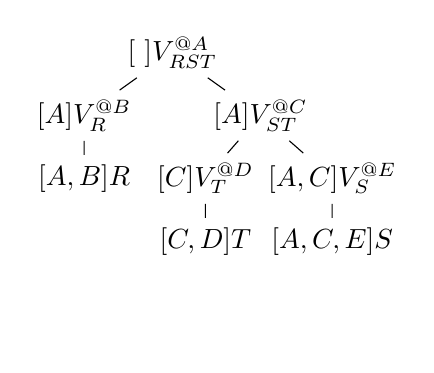
\begin{tikzpicture}[xscale=0.7, yscale=0.8]
      \node at (0, 0) (A) {$\VIEW[~]{V^{@A}_{RST}}$};
      \node at (-1.6, -1) (B) {$\VIEW[A]{V^{@B}_{R}}$} edge[-] (A);
      \node at (1.6, -1) (C) {$\VIEW[A]{V^{@C}_{ST}}$} edge[-] (A);
      \node at (0.6, -2) (D) {$\VIEW[C]{V^{@D}_{T}}$} edge[-] (C);
      \node at (2.9, -2) (E) {$\VIEW[A,C]{V^{@E}_{S}}$} edge[-] (C);
      
      \node at (-1.6, -2) {$\VIEW[A,B]{R}$} edge[-] (B);
      \node at (2.9, -3) {$\VIEW[A,C,E]{S}$} edge[-] (E);
      \node at (0.6, -3) {$\VIEW[C,D]{T}$} edge[-] (D);

      \node at (0.5, -4.5) {}; 
    \end{tikzpicture}
    % }
  \end{minipage}
  \begin{minipage}[b]{0.3\linewidth}
    \begin{align*}
      &\VIEW[A,C]{V^{@E}_{S}} = \VSUM_{E} \VIEW[A,C,E]{S} \\[2pt]
      &\VIEW[C]{V^{@D}_{T}} = \VSUM_{D} \VIEW[C,D]{T} \\[2pt]
      &\VIEW[~]{V^{@A}_{RST}} = \VSUM_{A} \big(\VIEW[A]{V^{@B}_{R}} \VPROD \VIEW[A]{V^{@C}_{ST}}\big) \\[2pt]
      &\VIEW[A]{V^{@B}_{R}} = \VSUM_{B} \VIEW[A,B]{R} \\[2pt]
      &\VIEW[A]{V^{@C}_{ST}} = \VSUM_{C} \big(\VIEW[C]{V^{@D}_{T}} \VPROD \VIEW[A,C]{V^{@E}_{S}}\big)
      \\[0.5cm]
   \end{align*}  
  \end{minipage}  
  \vspace*{-0.7cm}
\caption{
(left) Variable order $\omega$ of the natural join of the relations $\VIEW[A,B]{R}$, $\VIEW[A,C,E]{S}$, and $\VIEW[C,D]{T}$; (middle) View tree over $\omega$ and $\mathcal{F} = \emptyset$;
(right)  View definitions. 
}
\label{fig:example_payloads}
% \vspace*{-1em}
\end{figure}


%%%%%%%%%%%%%%%%%%%%%%%%%%%%%%%%%%%%

\paragraph{\textbf{Variable Orders.}}
Classical query evaluation makes use of  query plans that dictate the order in which the relations are joined. We use a different evaluation approach based on variable orders that dictate the  order in which we marginalize each join variable. This approach may require to join several relations at a time if they have the same variable. Our choice is motivated by the complexity of the evaluation problem for join queries: standard (relation-at-a-time) query plans are provably suboptimal, whereas the evaluation by variable orders can be worst-case optimal~\cite{Ngo:SIGREC:2013}.

Given a join query $Q$, a variable $X$ {\em depends} on a variable $Y$ if both are in the schema of a relation in $Q$.

\begin{definition}[adapted from \cite{Olteanu:FactBounds:2015:TODS}]\label{def:vo}
A {\em variable order} $\omega$ for a join query $Q$ is a pair $(F,dep)$, where $F$ is a rooted forest with one node per variable in $Q$, and {\em dep} is a function mapping each variable $X$ to a set of variables in $F$. It satisfies the following constraints:
\begin{itemize}
\item For each relation in $Q$, all of its variables lie along a root-to-leaf path in $F$.
%  
\item For each variable $X$, $dep(X)$ is the subset of its ancestors in $F$ on which the variables in the subtree rooted at $X$ depend.
\end{itemize}
\end{definition}

\begin{example}
Consider the query
%$\VIEW[~]{Q} = \VSUM_A\VSUM_B\VSUM_C\VSUM_D\VSUM_E \VIEW[A,B]{R}  \VPROD \VIEW[A,C,E]{S} \VPROD \VIEW[C,D]{T}$
from Example~\ref{ex:sql_count} that joins the relations $\VIEW{R}[A,B]$, $\VIEW[A,C,E]{S}$, and 
$\VIEW[C,D]{T}$.   
Figure~\ref{fig:example_payloads}  gives a variable order (top left) for
the query.
  Variable $D$ has ancestors $A$ and $C$, yet it only depends on $C$ since $C$ and $D$ appear in the same relation $\VIEW[]{T}$ and $D$ does not occur in any relation together with $A$. Thus, $dep(D)=\{C\}$. Given $C$, the variables $D$ and $E$ are independent of each other.
\punto
\end{example}
For a query $Q$ with free variables, a variable order is \emph{free-top} if no bound variable is an ancestor of a free variable~\cite{KNOZ20}. Variable orders are a different syntax~\cite{Olteanu:FactBounds:2015:TODS} for hypertree decompositions~\cite{Gottlob99}. They are more natural for algorithms that proceed one variable at a time.

%\paragraph{\textbf{View Trees.}}
\textbf{View Trees.} Our framework relies on a variable order $\omega$ for the input query $Q$ to describe the structure of the computation and indicate which variable marginalizations are pushed past joins. Based on $\omega$, we construct a tree of views that represent \DF's data structure to support query maintenance and enumeration.

\begin{figure}[t]
\centering
\setlength{\tabcolsep}{3pt}
\renewcommand{\arraystretch}{1.2}
\begin{tabular}{@{}c@{}c@{~~~}l}
  \toprule
  \multicolumn{3}{c}{$\tau$(\text{variable order} $\omega$, \text{free variables} $\mathcal{F}$) : view tree} \\
  \midrule
  \multicolumn{3}{l}{\MATCH $\omega$:} \\
  \midrule 
  \phantom{a} & $\VIEW{R}$\hspace*{1em} & \RETURN $\VIEW[\mathit{\sch(\VIEW{R})}]{R}$ \\
  \cmidrule{2-3} \\[-6pt] 
  &
  \begin{minipage}[b]{1.8cm}
    \begin{tikzpicture}[xscale=0.4, yscale=1]
      \node at (0,-2)  (n4) {$X$};
      \node at (-1,-3)  (n1) {$\omega_1$} edge[-] (n4);
      \node at (0,-3)  (n2) {$\ldots$};
      \node at (1,-3)  (n3) {$\omega_k$} edge[-] (n4);
      \node at (0,-4.5) {~};
    \end{tikzpicture}
    \vspace{1.5cm}
  \end{minipage}
  &
  \begin{minipage}[b]{6.3cm}
\LET $T_i = \tau(\omega_i, \mathcal{F}), \ \forall i\in[k] $\\[0.5ex]  
  \LET $\VIEW[\mathit{keys_i}]{V^{@\omega_i}_{rels_i}} = \text{ root of } T_i, \ \forall i\in[k] $\\[0.5ex]
    \LET $\mathit{keys}=\mathit{dep}(X) \cup (\mathcal{F} \cap \vars(\omega))$ \\[0.5ex]
    \LET $\mathsf{rels}=\bigcup_{i\in[k]}\mathsf{rels}_i$\\[0.5ex]
    \IF $X \notin \mathcal{F}$ \\[0.5ex]
    \TAB $\VIEW[\mathit{keys}]{V^{@X}_{rels}}= \VSUM_{X} \VPRODBIG_{i \in [k]} \VIEW[\mathit{keys_i}]{V^{@\omega_i}_{rels_i}}$\\[0.5ex]
    \ELSE \\[0.5ex]
    \TAB $\VIEW[\mathit{keys}]{V^{@X}_{rels}}=\VPRODBIG_{i \in [k]} \VIEW[\mathit{keys_i}]{V^{@\omega_i}_{rels_i}}$\\[0.5ex]
    \RETURN $
				\left\{
				\begin{array}{@{~~}c@{~~}}
					\tikz {
						\node at (1.2,-1)  (n4) {$\VIEW[\mathit{keys}]{V^{@X}_{rels}}$};
						\node at (0.8,-1.75)  (n1) {$T_1$} edge[-] (n4);
						\node at (1.25,-1.75)  (n2) {$\ldots$};
						\node at (1.8,-1.75)  (n3) {$T_k$} edge[-] (n4);
					}
				\end{array}  \right.$
  \end{minipage}
  \\
  \bottomrule
\end{tabular}
% \vspace*{-1em}
\caption{Creating a view tree $\tau(\omega, \mathcal{F})$ for a variable order $\omega$ and a set of free variables $\mathcal{F}$.}
\label{fig:static_view_tree_algo}
% \vspace*{-1.45em}
\end{figure}

Figure~\ref{fig:static_view_tree_algo} gives a function $\tau$ that constructs a view tree $\tau$ for a variable order $\omega$ and the set $\mathcal{F}$ of free variables of the query $Q$. Without loss of generality, we assume that $\omega$ is a single rooted tree. Otherwise, we apply $\tau$  to each tree in $\omega$ to obtain a set of view trees.
For simplicity, we assume that $\omega$ was first extended with relations as children under their lowest variable. 

The function  $\tau$ maps the variable order to a view tree of the same tree structure, yet with each variable $X$ replaced by a view $\VIEW[keys]{V^{@X}_{rels}}$. This notation states that the view $\VIEW{V}$ is (recursively) defined over the input relations {\sf rels}, has free variables $keys$, and it corresponds to the variable $X$ in $\omega$; in case of a view for an input relation $\VIEW{R}$, we use the simplified notation $\VIEW[\sch(\VIEW{R})]{R}$.

The base case (leaf in the extended variable order) is that of an input relation: We construct a view that is the relation itself. At a variable $X$ (inner node), we distinguish two cases: If $X$ is a bound variable, then we construct a view that marginalizes out $X$ in the natural join of the views that are children of the current view; we thus first join on $X$, then apply the lifting function for $X$ on its values, and aggregate $X$ away. If $X$ is a free variable, however, then we retain it in the view schema without applying the lifting function to its values. The schema of the view consists of $dep(X)$ and the free variables in the subtree of $\omega$ rooted at $X$.

\begin{figure}[t]
  \centering
  \begin{tikzpicture}
        \node at (0, 0.5) (x) {
    \begin{minipage}[b]{0.2\linewidth}
      \small
  %  \scalebox{0.95}{   
      \hspace{-0.25cm}
      \begin{tikzpicture}[xscale=0.8, yscale=0.24]  
        \node at (0, -1.5) (A) {$\VIEW[A,C]{V^{@A}_{RST}}$};
        \node at (-1.5, -5) (B) {$\VIEW[A]{V^{@B}_{R}}$} edge[-] (A);
        \node at (1.5, -5) (C) {$\VIEW[A,C]{V^{@C}_{ST}}$} edge[-] (A);
        \node at (0.5, -9) (D) {$\VIEW[C]{V^{@D}_{T}}$} edge[-] (C);
        \node at (2.5, -9) (E) {$\VIEW[A,C]{V^{@E}_{S}}$} edge[-] (C);
        
        \node at (-1.5, -8) {$\VIEW[A,B]{R}$} edge[-] (B);
        \node at (2.5, -12) {$\VIEW[A,C,E]{S}$} edge[-] (E);
        \node at (0.5, -12) {$\VIEW[C,D]{T}$} edge[-] (D);
  \end{tikzpicture}
  % }
    \end{minipage}
    };

        \node at (8.2, 0.5) (x) {
     \begin{minipage}[b]{0.3\linewidth}       
      % \scalebox{0.95}{\parbox{\linewidth}{%
        \begin{align*}
          &\VIEW[A,C]{V^{@A}_{RST}} = \VIEW[A]{V^{@B}_{R}} \VPROD \VIEW[A,C]{V^{@C}_{ST}} \\[2pt]
          &\VIEW[A,C]{V^{@C}_{ST}} = \VIEW[C]{V^{@D}_{T}} \VPROD \VIEW[A,C]{V^{@E}_{S}} \\[2pt]
          &\VIEW[A,C]{V^{@E}_{S}} = \VSUM_{E} \VIEW[A,C,E]{S} \\[2pt]
          &\VIEW[A]{V^{@B}_{R}} =  \VSUM_{B}\VIEW[A,B]{R} \\[2pt]
          &\VIEW[C]{V^{@D}_{T}} =  \VSUM_{D}\VIEW[C,D]{T}
        \end{align*}
      % }}    
    \end{minipage}
};
\end{tikzpicture}    
  \caption{
  (left) View tree over the variable order $\omega$ in Figure~\ref{fig:example_payloads} and 
  $\mathcal{F} = \{A,C\}$; (right) View definitions.
  }
  \label{fig:view tree_free_vars}
  % \vspace*{-1em}
\end{figure}

\begin{figure}[t]
  \begin{minipage}[b]{\linewidth}
    \centering
    \small
    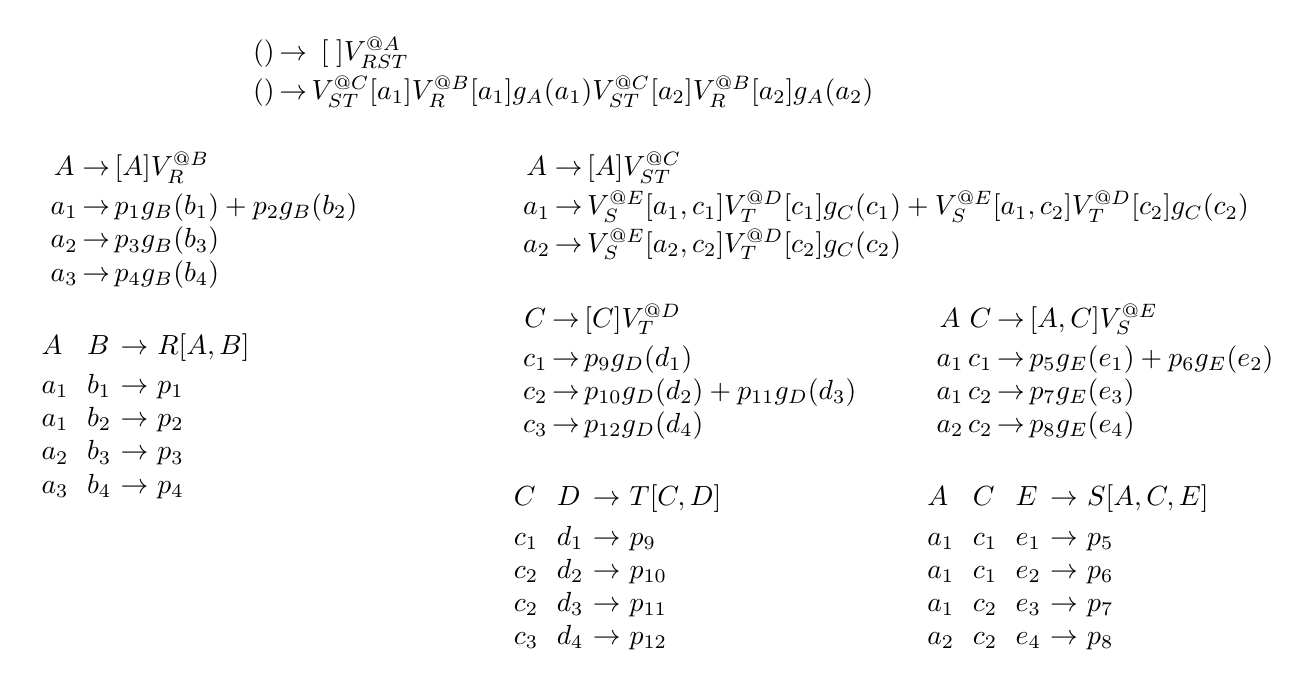
\begin{tikzpicture}[xscale=0.75, yscale=0.35]         
    
      % at node A
      \node at (2, 0) {
        \begin{tabular}{@{\,}l@{\,}  @{\,}c@{\,}c@{\,}l@{\,}}
          & $()$ & $\rightarrow$ & \ $\VIEW[\;]{V^{@A}_{RST}}$ \\[0.5ex]\toprule
          & $()$ & $\rightarrow$ & 
          $\VIEW{V^{@C}_{ST}}[a_1] \RINGPROD \VIEW{V^{@B}_{R}}[a_1] \RINGPROD g_A(a_1) \RINGPLUS \VIEW{V^{@C}_{ST}}[a_2] \RINGPROD \VIEW{V^{@B}_{R}}[a_2] \RINGPROD g_A(a_2) $           
          \\\bottomrule
        \end{tabular}
      };   

      % at node B
      \node[anchor=north west] at (-7, -2.5) {
        \begin{tabular}{@{\,}l@{\,} @{\,}c@{\,}c@{\,}l@{\,}}
          %  
          & $A$ & $\to$ & $\VIEW[A]{V^{@B}_{R}}$ \\[0.5ex]\toprule
          & $a_1$ & $\rightarrow$ & $p_{1} \RINGPROD  g_B(b_1)  + p_{2} \RINGPROD  g_B(b_2)$ \\
          & $a_2$ & $\rightarrow$ & $p_{3} \RINGPROD  g_B(b_3)$ \\
          & $a_3$ & $\rightarrow$ & $p_{4} \RINGPROD  g_B(b_4)$\\\bottomrule
        \end{tabular}
      };
      
      % at node R
      \node[anchor=north west] at (-7, -9) {
      \begin{tabular}{@{\,}l@{~~}l@{~$\to$~}l@{\,}}
        $A$ & $B$ & $\VIEW{R}[A,B]$\\[0.5ex]\toprule
        $a_1$ & $b_1$ & $p_1$ \\
        $a_1$ & $b_2$ & $p_2$\\  
        $a_2$ & $b_3$ & $p_3$\\
        $a_3$ & $b_4$ & $p_4$\\\bottomrule
        \end{tabular}
      };

      % at node C
      \node [anchor=north west] at (1, -2.5) {
        \begin{tabular}{@{\,}l@{\,} @{\,}c@{\,}c@{\,}l@{\,}}
          & $A$ & $\rightarrow$ & $\VIEW[A]{V^{@C}_{ST}}$ \\[0.5ex]\toprule
          & $a_1$ & $\rightarrow$ & 
          $\VIEW{V^{@E}_{S}}[a_1,c_1] \RINGPROD \VIEW{V^{@D}_{T}}[c_1] \RINGPROD g_C(c_1) + 
          \VIEW{V^{@E}_{S}}[a_1,c_2] \RINGPROD \VIEW{V^{@D}_{T}}[c_2] \RINGPROD g_C(c_2)$ \\[0.05cm]  
          & $a_2$ & $\rightarrow$ & $\VIEW{V^{@E}_{S}}[a_2,c_2] \RINGPROD \VIEW{V^{@D}_{T}}[c_2] \RINGPROD g_C(c_2)$ \\
          \bottomrule 
        \end{tabular}
      };

      % at node D
      \node [anchor=north west] at (1, -8) {
        \begin{tabular}{@{\,}l@{\,} @{\,}c@{\,}c@{\,}l@{\,}}
          %  
          & $C$ & $\to$ & $\VIEW[C]{V^{@D}_{T}}$ \\[0.5ex]\toprule
          & $c_1$ & $\rightarrow$ & $ p_9 \RINGPROD g_D(d_1)$\\
          & $c_2$ & $\rightarrow$ & $p_{10} \RINGPROD  g_D(d_2)  + p_{11} \RINGPROD  g_D(d_3)$ \\
          & $c_3$ & $\rightarrow$ & $p_{12} \RINGPROD  g_D(d_4)$ \\\bottomrule
        \end{tabular}
      };

      % at node E
      \node [anchor=north west] at (8, -8) {
        \begin{tabular}{@{\,}l@{\,} @{\,}c@{\,}c@{\,}c@{\,}l@{\,}}
          & $A$ & $C$ & $\to$ & $\VIEW[A,C]{V^{@E}_{S}}$ \\[0.5ex]\toprule
          & $a_1$ & $c_1$ & $\rightarrow$ & $p_{5} \RINGPROD  g_E(e_1)  + p_{6} \RINGPROD  g_E(e_2)$ \\
          & $a_1$ & $c_2$ & $\rightarrow$ & $p_{7} \RINGPROD  g_E(e_3)$  \\
          & $a_2$ & $c_2$ & $\rightarrow$ & $p_{8} \RINGPROD  g_E(e_4) $ \\\bottomrule
        \end{tabular}
      };
      
      % at node T
      \node [anchor=north west] at (1, -14.5) {
       \begin{tabular}{@{\,}l@{~~}l@{~$\to$~}l@{\,}}
        $C$ & $D$ & $\VIEW{T}[C,D]$ \\[0.5ex]\toprule
        $c_1$ & $d_1$ & $p_9$\\
        $c_2$ & $d_2$ & $p_{10}$\\
        $c_2$ & $d_3$ & $p_{11}$\\
        $c_3$ & $d_4$ & $p_{12}$\\\bottomrule
      \end{tabular}
      };

      % at node S
      \node [anchor=north west] at (8, -14.5) {
      \begin{tabular}{@{\,}l@{~~}l@{~~}l@{~$\to$~}l@{\,}}
        $A$ & $C$ & $E$ & $\VIEW{S}[A,C,E]$ \\[0.5ex]\toprule
        $a_1$ & $c_1$ & $e_1$ & $p_5$\\
        $a_1$ & $c_1$ & $e_2$ & $p_6$\\
        $a_1$ & $c_2$ & $e_3$ & $p_7$\\
        $a_2$ & $c_2$ & $e_4$ & $p_8$\\\bottomrule
      \end{tabular}
      };
    \end{tikzpicture}
  \end{minipage}
\caption{
Contents of the views in the view tree from Figure~\ref{fig:example_payloads} in case the relations 
$\VIEW{R}$,
$\VIEW{S}$, and $\VIEW{T}$ are over a ring 
$(\RING, \RINGPLUS, \RINGPROD, \RINGZERO, \RINGONE)$ with $p_i \in \RING$ for
$i \in [12]$.}
\label{fig:count}
\end{figure}

\begin{example}
\label{ex:views_count}
Figure~\ref{fig:example_payloads} shows the view tree constructed by the function $\tau$ from 
Figure~\ref{fig:static_view_tree_algo} over the variable order $\omega$ and the empty set of free variables.
Figure~\ref{fig:view tree_free_vars} depicts 
  the view tree constructed over the
  same variable order but for 
the set  $\mathcal{F} = \{A,C\}$ of free variables.
  
Figure~\ref{fig:count} gives the  
  contents of the views in the view tree from Figure~\ref{fig:example_payloads}, where 
$\VIEW{R}$,
$\VIEW{S}$, and $\VIEW{T}$ are relations over a ring $\RING$ with payloads $p_i \in \RING$ for
$i \in [12]$. 
Assume that $\RING$ is the $\mathbb{Z}$ ring, 
each tuple in these relations 
is mapped to $1$,
i.e.,  $p_i = 1$ for $i \in [12]$, and 
the lifting functions map all
values to $1$.
Then, the view tree 
computes the {\tt COUNT} query 
from Example~\ref{ex:sql_count}
and the root view $\VIEW{V_{RST}^{@A}}$ maps the empty tuple to 
  the overall count $10$,
which is the number 
of tuples in the natural join of $\VIEW{R}$, $\VIEW{S}$, and 
$\VIEW{T}$.
\punto
\end{example}

By default, the function $\tau$ in Figure~\ref{fig:static_view_tree_algo} constructs one view per variable in the variable order $\omega$. A wide relation (with many variables) leads to long branches in $\omega$ with variables that are only local to this relation. This is, for instance, the case of our retailer dataset used in 
Section~\ref{sec:experiments}. Such long branches create long chains of views, where each view marginalizes one bound variable over its child view in the chain. For practical reasons, we compose such long chains into a single view that marginalizes several variables at a time. 

  